\section{Supporting Info}
\graphicspath{{./chapters/c3_binfree/si_figure/}}

\section*{Transient Binding sample preparation}


\section*{Binned time traces dependence with bin time}



\section*{Lipid bilayer sample preparation}



\section*{2D Numerical simulations}

The current program is organized in only one script, simualtion2d.m and contains several subroutines. It also uses the program generate\_simulation\_parameters.m to set all the needed parameters for the simulation. These are divided in two sets, the physical parameters and the simulation parameters. 
The former set of parameters corresponds to the experimentally relevant variables while the latter corresponds to the extra parameters needed to run the simulation and are not related to the experimental conditions but need to be selected to run the simulation. 
The output of the program is a structure that has contains the unbinned time traces, binned time traces and interphoton histograms. The physical inputs are the following: concentration of molecules $C$, intensity distribution of the incoming beam $I(\ve{r})$ and dark counts of the detector $Dc$. 
For a complete list of the simulation parameters, refer to the appendix \ref{ap:sim_param}.

The calculation consists of several steps that will be summarized in the following. 
The spatial intensity distribution input has to be a matrix $M$ with the spatial intensity distribution of the incoming beam $I(\ve{r})$ (in cps). 
The first step is done by the subroutine \texttt{calculate\_times} to simulate the absolute arrival photon times for each intensity value of the matrix 
\footnote{This can be improved in speed by not calculating the repeated intensity values more than one time and by saving the output structure in a file and loading it later instead of recalculating it.} 
within the time of the experiment, $T_{\mbox{Max}}$. This traces correspond to a single molecule placed in each pixel of the intensity matrix.
To generate the correct exponential distribution for a given intensity $I$, I use the fact that the interphoton times should follow an exponential distribution:
\begin{equation}
\Delta t_{i} = -\frac{\log\left(\zeta_i \right)}{I} \, ,
\label{eq:interphoton_simulation}
\end{equation}
where $\Delta t_{i}$ ($i=0,...,N$) represents the time between successive photons detection and $\zeta_i$ is a random number in the interval $(0,1)$. 
This way of generating the interphoton times ensures the required exponential distribution. Then by performing the cumulative sum over the interphoton times the absolute arrival times of the simulated stream of photons can be calculated for each intensity value in the input intensity matrix $M$. This data is contained in a structure named \texttt{abs\_times}. 

The next step is to calculate the number of molecules present in the simulation volume  $V_{sim}$. For a given concentration, the number of molecules contributing to the simulation is random variable that follows Poisson distribution with a mean value $\left<N_{molecules}\right> = C V_{sim}$. Since our calculation is based on the calculation of the interphoton arrival time for a fixed number of molecules $N_{molecules}$ in the simulation volume, we calculate the number of molecules needed to contain 99\% of the cases. Then, for each $N_{molecules}$ we generate the interphoton histogram as follows. We generate random positions for all the available molecules in the simulation volume and we retrieve the corresponding absolute photon arrival times from the variable abs\_times. We concatenate all this arrival time and also include extra photon detections generated by the dark counts of the detector. The mean number of dark photons in the simulation time is $Dc T_{\mbox{max}}$ and follows a poisson distribution. We use a poissonian number generator to simulate the number of detected photons in each run and then distribute them uniformly in the time trace. All this concatenated absolute photon detection times are then sorted and saved in a vector $t$. Then the histogram of the interphoton times for this vector is computed, using pre-fixed bins (with a certain number of points $Hist_{\mbox{Npts}}$) . The normalized (to the total counts) histogram is stored into the first component of a matrix of histogram counts $H$. Then we repeat this procedure $N_{\mbox{config}}$ time, using each time a new set of random positions for all the molecules, creating the matrix of dimensions $Hist_{\mbox{Npts}} \times N_{\mbox{config}}$. Then we average the normalized histograms corresponding to different spatial configurations, contained in $H$ to obtain a single histogram corresponding for a single number of molecules in the simulation volume. The final step is to perform a weighted average of the histograms for each number of molecules contributing to the simulation for a fixed concentration using the corresponding poissonian weight.



\section*{Slow diffusion case}

We simulated the case of a molecule 


\section*{Simulation Parameters\label{ap:sim_param}}

\section*{code validation\label{ap:code}}

In order to validate the simulation code we tested the results with a simple beam shape that provides an analytical solution. 
We work in two dimensions just for simplicity with a rectangular beam shape with constant intensity and zero intensity outside, described mathematically as:
\begin{equation}
I(x,y) = I_0\theta(|x-\frac{x_0}{2}|)\theta(|y-\frac{y_0}{2}|)\, ,
\label{eq:theta_intensity}
\end{equation}
with $I_0$ the maximum intensity and $x_0,y_0$ the size in lateral directions and $\theta(\zeta)$ the step function. Thus, the illuminated area has a volume of $V_0=x_0y_0$. 
For such a beam shape the interphoton probability distribution can be obtained by simple integration of equation \ref{eq:result} replacing the beam shape $I(\ve{r})$ with equation \ref{eq:theta_intensity}, obtaining
\begin{equation}
p(\tau) = I_0 C V_0 \exp[-\tau I_0-C V_0(1-\exp(-\tau I_0))]\,.
\label{eq:theta_interphoton_distribution}
\end{equation}

Figure \ref{fg:square_beam}(a) shows an example in a particular case when the dimensions are the same for the two directions and \ref{fg:square_beam}(b) shows plots for the analytical solution for different intensities and concentrations.




 \begin{figure}
 \centering
 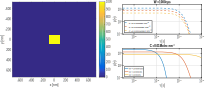
\includegraphics[width=\textwidth]{square_illumination}%
 \caption{\textbf{Simple illumination profile that provides an analytical solution to test the simulation code} 
(a) Colormap plot of the square-shaped beam we use for validating the code. We used $x_0=y_0=182$ nm and $I_0=1000$ cps.
(b)Analytical plots of the interphoton probability distribution for different intensities and concentrations. 
\label{fg:square_beam}}
 \end{figure}


%\figdouble{square_illumination}{square_illumination_analytical}{fg:square_beam}{Simple illumination profile that provides an analytical solution to test the simulation code}{ \figa Colormap plot of the square-shaped beam we use for validating the code. We used $x_0=y_0=182$ nm and $I_0=1000$ cps. \figb }


In order to test the code we performed simulations using this illumination distribution and compared it with the analytical result. We started with a fixed superficial concentration  C=$2 \times 10^{-4}$ molecules nm$^2$ to have a relative fast run and we changed the different parameters of the simulation, such as the number of spatial configurations to average and the total simulation time $T_{\mbox{max}}$. The comparison with the analytical curves can be seen in figure \ref{fg:sim_test}. In both cases the simulation agrees well with the analytical result and for longer simulation time or higher number of configurations, the error becomes smaller.


 \begin{figure}
 \centering
 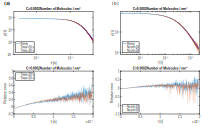
\includegraphics[width=\textwidth]{Theta_results}%
 \caption{\textbf{Test of simulation parameters and code validation} 
(a) Different total simulation times. Top: simulated and analytical curves. Bottom: relative error in the simulation.
(b) Different number of averaged spatial configurations. Top: simulated and analytical curves for different total simulation times $T_{\mbox{max}}$. Bottom: relative error in the simulation.
\label{fg:Theta_results}}
 \end{figure}


The next step was to test the simulation for different physical parameters such as the concentration of molecules and the intensity in the beam. The results for three different concentrations and intensities can be found in figure \ref{fg:phy_test}. The results again agree with the analytical curves and it can be noted that the larger the number of photons generated in the simulation the better correspondence with the analytical result.


 \begin{figure}
 \centering
 \includegraphics[width=\textwidth]{Theta_physical_test}%
 \caption{\textbf{Test of physical parameters and code validation} 
(a) Different concentrations. Top: simulated and analytical curves. Bottom: relative error in the simulation.
(b) Different intensities. Top: simulated and analytical curves. Bottom: relative error in the simulation.
\label{fg:Theta_physical_test}}
 \end{figure}